\section{Example Objects}

Totally tubular examples.  We are making

\subsection{Touch-sensitive Toy}

\begin{figure}[h]
\centering
    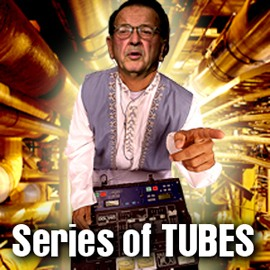
\includegraphics[width=3.4in]{figures/series-of-tubes.jpg}
\caption{A touch-sensitive rabbit whose tubes are filled with conductive paint.  Sensing is done on a single wire via SFCS.  Inset shows the internal structure of the tubes generated by our design tool.}
\label{fig:toy}
\end{figure}

We created a touch-sensitive toy and an app that goes along with it, reminiscent of the boat application in \cite{Harrison-acoustic}.  This toy has an interior star topology where a single wire attached to an Arduino running an SFCS sketch splits to connect to sensors on the eyes, ears, tail, and nose.  To accompany this toy, we built an app which prompts the user to find and touch certain parts of the animal (see Figure \ref{fig:toy}).

\subsection{Braille Haptic Display}

\begin{figure}[h]
\centering
    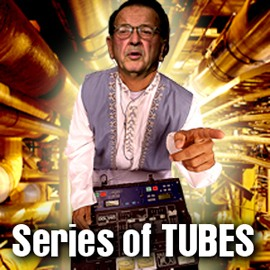
\includegraphics[width=3.4in]{figures/series-of-tubes.jpg}
\caption{When air pressure is changed in the six tubes, their caps inflate or deflate. Through controlled actuation, we can create Braille letters.  Inset shows the internal structure of the tubes generated by our design tool.}
\label{fig:braille}
\end{figure}

Using a $2\times3$ array of semi-closed tubes, we created a Braille output interface.  The closed ends of the tubes are covered in a rubberlike material, while on the system side the tubes are attached to individually-controlled air pumps.  These pumps can create positive or negative pressure in each tube, pushing the cap up or down and rendering a tactile Braille letter when used in concert (see Figure \ref{fig:braille}).

\subsection{Custom Radio}

\begin{figure}[h]
\centering
    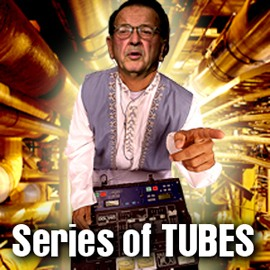
\includegraphics[width=3.4in]{figures/series-of-tubes.jpg}
\caption{This radio is assembled from traditional electronic components connected by copper-filled tubes.  The case was designed to allow the components to recess into it slightly.  Inset shows the internal structure of the tubes generated by our design tool.}
\label{fig:radio}
\end{figure}

A custom ``radio'' built using tubes allows users to tune to different stations and play sound files related to those stations.  This device uses a network of disconnected open tubes filled with conductive paint to connect traditional electronic components (a potentiometer, a piezo, and an LED) to a microcontroller.

\subsection{Presence-aware Pen Holder}

\begin{figure}[h]
\centering
    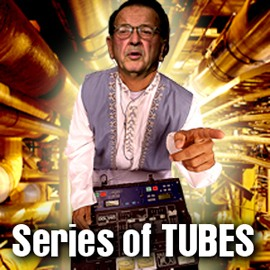
\includegraphics[width=3.4in]{figures/series-of-tubes.jpg}
\caption{This pen holder (a) uses the FlyEye technique (b) to sense the presence or absence of an object in each of its tubes.  Inset shows the internal structure of the tubes generated by our design tool.}
\label{fig:pens}
\end{figure}

Our presence-aware pen holder can distinguish which tool or tools a user has picked up (see Figure \ref{fig:pens}).  Such information was used by \cite{Mueller-constructable} to determine which physical laser pointer a designer was using to interact with their interface.  Our pen holder uses the FlyEye technique described by Wimmer in \cite{Wimmer-flyeye} and contains open tubes filled with fiber optic cables, two per pen chamber.  One tube from each chamber leads to an infrared LED, and the other leads to a camera.  When a pen is in its appointed place, light from the LED is reflected off its bottom and travels through the other optical fiber into the camera, where it registers as a bright point.  A dark point on the camera region appears when a pen has been removed from its place, and the position of the point indicates which pen it is.

\subsection{Animated Neon Sign}

\begin{figure}[h]
\centering
    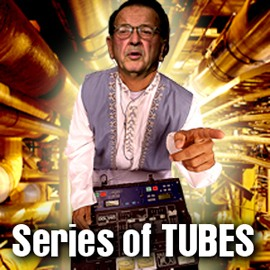
\includegraphics[width=3.4in]{figures/series-of-tubes.jpg}
\caption{A neon sign (a) and its partial duplicate designed using our tool (b).  (c) shows the selections we made to generate our tube structures.  (d) shows the internal structure of the tubes generated by our design tool.}
\label{fig:neon}
\end{figure}

Neon art, perhaps best known for its association with Las Vegas, is traditionally made from hand-formed glass tubes containing neon gas.  The tubes light up when a current is passed through them.  For this type of art, the path of the tubes is of crucial importance, as it determines how the sign will look.  We designed a partial duplicate of a renowned piece of neon art from Seattle (or was it Portland?).  The piece features open tubes due to support-flushing constraints, however the tubes could also be semi-closed.  They have been threaded with EL wire which is lit in sequence to create an animation.